% 图 73.3 —— 由 `checks/emit_hand.py` 自动拼出（probe 精测 + prims2 图元分解）
%%
% ⚠ 这是**稿子不是成品**：跑 `checks/checkhand.py 73.3` 看指标 + 看叠合图。
%%
%% ⚠ 待核：
%   · 本图 probe 报出阴影族 2 个 —— **本脚本不生成阴影**（要照原书手写）；prims2 的 strokes 里可能含阴影线，核对时留意别画重
%   · 可疑字形 6 项（空心圈 ⊙ 常被认成字母 o）—— 见文件末
%%
\documentclass[12pt]{standalone}
\usepackage{fontspec}
\setsansfont{Arial}
\newfontfamily\mfallback{DejaVu Sans}
\usepackage{tikz}
\begin{document}
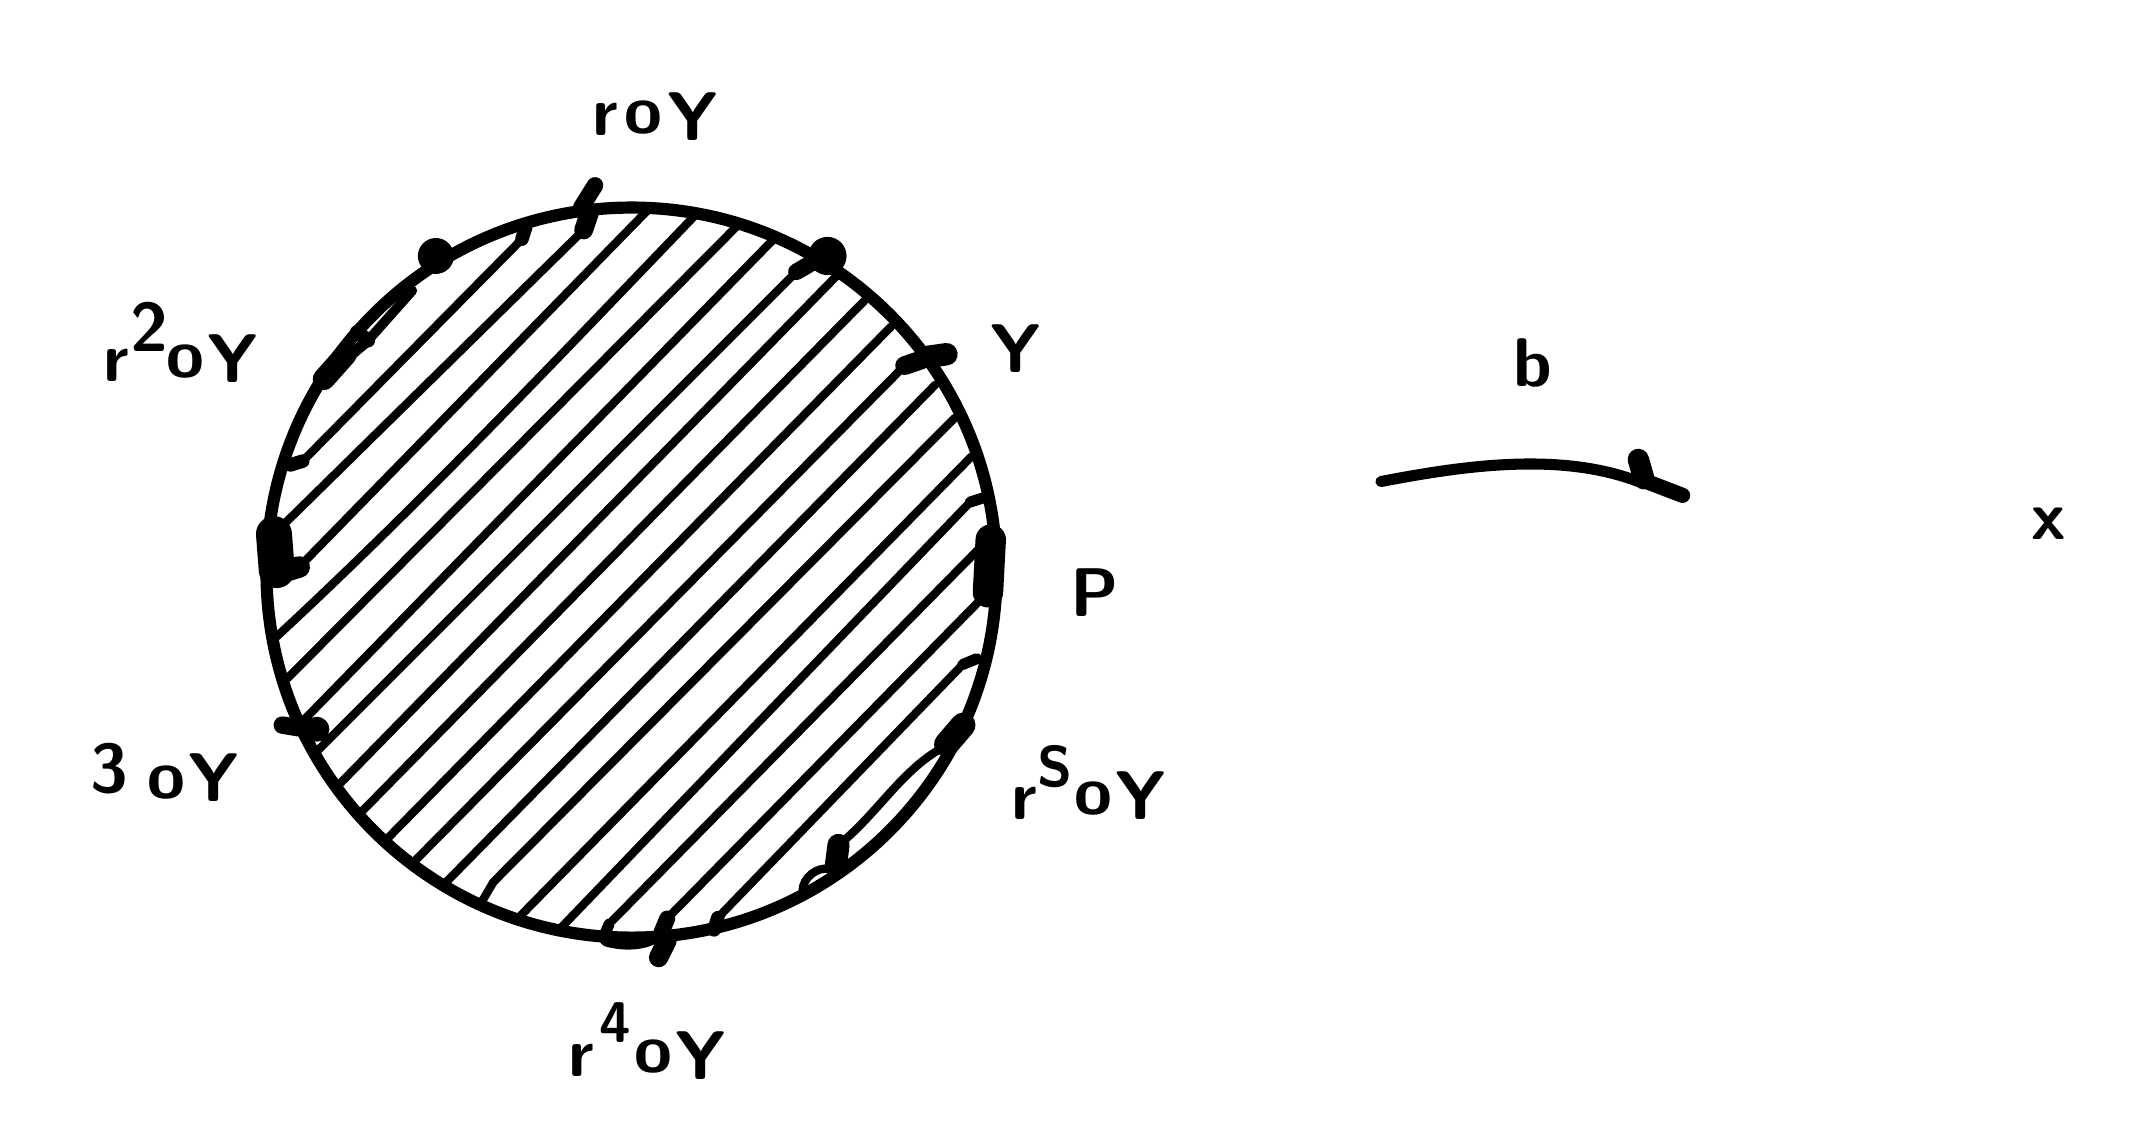
\begin{tikzpicture}[x=1pt, y=-1pt, line width=4.4pt, line cap=round, line join=round]

  %% ════ 填充区（prims2 的 fills）════

  %% ════ 直线段（prims2 的 strokes）════
  \draw[line width=3.5pt] (139.0,95.0) -- (123.0,113.0);
  \draw[line width=8.0pt] (107.0,127.0) -- (115.0,118.0);
  \draw[line width=3.0pt] (256.0,72.0) -- (94.0,235.0);
  \draw[line width=6.0pt] (285.0,84.0) -- (277.8,88.2);
  \draw[line width=3.0pt] (277.8,88.2) -- (105.0,261.0);
  \draw[line width=8.1pt] (332.0,118.0) -- (325.0,119.0);
  \draw[line width=13.0pt] (90.0,196.0) -- (89.0,183.0);
  \draw[line width=3.0pt] (99.0,251.0) -- (269.0,77.0);
  \draw[line width=3.0pt] (224.0,66.0) -- (98.1,194.9);
  \draw[line width=7.8pt] (98.1,194.9) -- (91.0,197.0);
  \draw[line width=5.5pt] (585.0,164.0) -- (598.0,169.0);
  \draw[line width=3.0pt] (164.0,316.0) -- (168.3,308.7);
  \draw[line width=3.0pt] (168.3,308.7) -- (335.0,141.0);
  \draw[line width=6.8pt] (323.0,120.0) -- (316.9,122.1);
  \draw[line width=3.0pt] (316.9,122.1) -- (139.0,302.0);
  \draw[line width=4.0pt] (345.0,170.0) -- (340.6,171.4);
  \draw[line width=3.0pt] (340.6,171.4) -- (192.0,326.0);
  \draw[line width=3.0pt] (177.0,322.0) -- (341.0,155.0);
  \draw[line width=3.0pt] (90.0,182.0) -- (200.9,73.1);
  \draw[line width=6.8pt] (200.9,73.1) -- (203.0,67.0);
  \draw[line width=6.0pt] (200.0,65.0) -- (205.0,57.0);
  \draw[line width=4.0pt] (343.0,228.0) -- (337.9,230.1);
  \draw[line width=3.0pt] (337.9,230.1) -- (249.4,321.6);
  \draw[line width=4.9pt] (249.4,321.6) -- (248.0,326.0);
  \draw[line width=6.3pt] (98.0,253.0) -- (92.0,252.0);
  \draw[line width=4.0pt] (117.0,118.0) -- (123.0,113.0);
  \draw[line width=3.0pt] (347.0,185.0) -- (210.1,323.9);
  \draw[line width=4.0pt] (210.1,323.9) -- (208.0,329.0);
  \draw[line width=4.9pt] (180.0,72.0) -- (178.6,76.4);
  \draw[line width=3.0pt] (178.6,76.4) -- (99.4,156.6);
  \draw[line width=4.9pt] (99.4,156.6) -- (95.0,158.0);
  \draw[line width=8.0pt] (293.0,295.3) -- (292.0,303.0);
  \draw[line width=7.0pt] (231.0,330.0) -- (228.0,336.0);
  \draw[line width=11.0pt] (347.0,204.0) -- (348.0,185.0);
  \draw[line width=7.7pt] (584.0,163.0) -- (582.0,156.0);
  \draw[line width=3.0pt] (346.0,205.0) -- (231.1,321.9);
  \draw[line width=5.8pt] (231.1,321.9) -- (229.0,327.0);
  \draw[line width=3.0pt] (120.0,284.0) -- (303.0,98.0);
  \draw[line width=3.0pt] (312.0,108.0) -- (130.0,293.0);
  \draw[line width=3.0pt] (328.0,129.0) -- (151.0,309.0);
  \draw[line width=3.0pt] (292.0,90.0) -- (113.0,273.0);
  \draw[line width=5.1pt] (123.0,113.0) -- (119.0,110.0);
  \draw[line width=9.0pt] (338.0,252.0) -- (332.0,259.0);

  %% ════ 曲线（prims2 的 curves —— 三段式，坐标同为 (y,x)）════
  \draw[line width=3.0pt] (90.0,220.0) .. controls (142.9,171.0) and (191.4,119.5) .. (241.0,68.0);
  \draw[line width=4.0pt] (209.0,330.0) .. controls (214.9,331.7) and (223.0,331.8) .. (228.0,328.0);
  \draw[line width=4.0pt] (489.0,164.0) .. controls (518.2,158.4) and (553.5,153.1) .. (582.0,164.0);
  \draw[line width=3.0pt] (331.0,260.0) .. controls (316.0,267.8) and (306.5,284.8) .. (293.0,295.3);
  \draw[line width=3.0pt] (280.0,312.0) .. controls (280.0,307.2) and (285.2,303.0) .. (290.0,304.0);

  %% ════ 圆 / 椭圆（probe 精测）════
  \draw (218.2,196.9) circle (131.9);

  %% ════ 实心点 ════
  \fill (147.5,82.5) circle (6.5);
  \fill (289.0,82.5) circle (6.9);
  \fill (104.5,253.5) circle (4.5);

  %% ════ 标签（probe 直接给的 \node 行）════
  %% ⚠ 全部补了 fill=white：文字在最上层，否则与曲线交叉干扰
     \node[anchor=center,inner sep=0pt,fill=white,font=\fontsize{28.7}{35.9}\selectfont] at (240.5,32.0) {\textsf{\textbf{\textit{Y}}}};   % box(232,19,16,24)
     \node[anchor=center,inner sep=0pt,fill=white,font=\fontsize{32.1}{40.1}\selectfont] at (208.9,33.4) {\textsf{\textbf{\textit{r}}}};   % box(200,23,14,17)
     \node[anchor=center,inner sep=0pt,fill=white,font=\fontsize{23.1}{28.8}\selectfont] at (222.6,32.7) {\textsf{\textbf{\textit{o}}}};   % box(216,25,12,13)
     \node[anchor=center,inner sep=0pt,fill=white,font=\fontsize{22.9}{28.7}\selectfont] at (44.1,108.4) {\textsf{\textbf{2}}};   % box(38,100,11,16)
     \node[anchor=center,inner sep=0pt,fill=white,font=\fontsize{28.7}{35.9}\selectfont] at (357.5,116.0) {\textsf{\textbf{\textit{Y}}}};   % box(349,103,16,24)
     \node[anchor=center,inner sep=0pt,fill=white,font=\fontsize{29.3}{36.6}\selectfont] at (74.5,119.5) {\textsf{\textbf{\textit{Y}}}};   % box(66,106,16,25)
     \node[anchor=center,inner sep=0pt,fill=white,font=\fontsize{30.0}{37.5}\selectfont] at (543.8,121.2) {\textsf{\textbf{\textit{b}}}};   % box(534,109,17,22)
     \node[anchor=center,inner sep=0pt,fill=white,font=\fontsize{30.9}{38.7}\selectfont] at (32.3,122.3) {\textsf{\textbf{\textit{r}}}};   % box(24,112,13,17)
     \node[anchor=center,inner sep=0pt,fill=white,font=\fontsize{24.0}{30.0}\selectfont] at (57.1,120.7) {\textsf{\textbf{\textit{o}}}};   % box(50,113,13,13)
     \node[anchor=center,inner sep=0pt,fill=white,font=\fontsize{35.3}{44.1}\selectfont] at (730.2,179.4) {\textsf{\textbf{\textit{x}}}};   % box(720,166,18,22)
     \node[anchor=center,inner sep=0pt,fill=white,font=\fontsize{30.0}{37.4}\selectfont] at (385.5,204.0) {\textsf{\textbf{\textit{P}}}};   % box(374,192,19,22)
     \node[anchor=center,inner sep=0pt,fill=white,font=\fontsize{44.3}{55.4}\selectfont] at (29.7,267.6) {\textsf{\textbf{3}}};   % box(17,252,24,29)
     \node[anchor=center,inner sep=0pt,fill=white,font=\fontsize{28.7}{35.9}\selectfont] at (67.5,271.0) {\textsf{\textbf{\textit{Y}}}};   % box(59,258,16,24)
     \node[anchor=center,inner sep=0pt,fill=white,font=\fontsize{20.6}{25.8}\selectfont] at (371.3,267.0) {\textsf{\textbf{\textit{S}}}};   % box(366,258,11,17)
     \node[anchor=center,inner sep=0pt,fill=white,font=\fontsize{29.3}{36.6}\selectfont] at (402.5,277.5) {\textsf{\textbf{\textit{Y}}}};   % box(394,264,16,25)
     \node[anchor=center,inner sep=0pt,fill=white,font=\fontsize{24.0}{30.0}\selectfont] at (50.1,272.7) {\textsf{\textbf{\textit{o}}}};   % box(43,265,13,13)
     \node[anchor=center,inner sep=0pt,fill=white,font=\fontsize{30.9}{38.7}\selectfont] at (360.3,280.3) {\textsf{\textbf{\textit{r}}}};   % box(352,270,13,17)
     \node[anchor=center,inner sep=0pt,fill=white,font=\fontsize{24.0}{30.0}\selectfont] at (385.1,278.7) {\textsf{\textbf{\textit{o}}}};   % box(378,271,13,13)
     \node[anchor=center,inner sep=0pt,fill=white,font=\fontsize{21.8}{27.3}\selectfont] at (212.2,359.4) {\textsf{\textbf{4}}};   % box(206,351,11,16)
     \node[anchor=center,inner sep=0pt,fill=white,font=\fontsize{29.3}{36.6}\selectfont] at (243.5,371.5) {\textsf{\textbf{\textit{Y}}}};   % box(235,358,16,25)
     \node[anchor=center,inner sep=0pt,fill=white,font=\fontsize{30.9}{38.7}\selectfont] at (200.3,373.3) {\textsf{\textbf{\textit{r}}}};   % box(192,363,13,17)
     \node[anchor=center,inner sep=0pt,fill=white,font=\fontsize{24.0}{30.0}\selectfont] at (226.1,371.7) {\textsf{\textbf{\textit{o}}}};   % box(219,364,13,13)

  % 钉死画布：否则超出的图元/控制点会把页面撑大，1:1 回比就失准
  \pgfresetboundingbox
  \path[use as bounding box] (0,0) rectangle (750,393);
\end{tikzpicture}
\end{document}

% ⚠ 待核清单（probe 拿不准，人眼过一遍）：
%   · 可疑字形：\node[anchor=center,inner sep=0pt,font=\fontsize{23.1}{28.8}\selectfont] at (222.6,32.7) {\textsf{\textbf{\tex
%   · 可疑字形：\node[anchor=center,inner sep=0pt,font=\fontsize{24.0}{30.0}\selectfont] at (57.1,120.7) {\textsf{\textbf{\tex
%   · 可疑字形：\node[anchor=center,inner sep=0pt,font=\fontsize{24.0}{30.0}\selectfont] at (50.1,272.7) {\textsf{\textbf{\tex
%   · 可疑字形：\node[anchor=center,inner sep=0pt,font=\fontsize{24.0}{30.0}\selectfont] at (385.1,278.7) {\textsf{\textbf{\te
%   · 可疑字形：\node[anchor=center,inner sep=0pt,font=\fontsize{24.0}{30.0}\selectfont] at (226.1,371.7) {\textsf{\textbf{\te
%   · 未识别/跳过：⑤ 跳过/未识别的字形
